\documentclass[11pt]{article}
\usepackage{array, xcolor}
\usepackage[margin=1.5cm]{geometry}
\usepackage{hyperref}

\usepackage{graphicx,mwe}
\usepackage{array}
\usepackage{graphicx}
\usepackage{wrapfig}

\usepackage{enumitem}

\usepackage{fontspec}
\defaultfontfeatures{Scale=MatchLowercase,Mapping=tex-text}
\setmainfont[Ligatures=TeX]{DejaVu Serif}
\setsansfont[Ligatures=TeX]{DejaVu Sans}
\setmonofont{DejaVu Sans Mono}
 
 \usepackage[none]{hyphenat}
  
\title{\bfseries\Huge Oleg Shpynov}
\author{oshpynov@wustl.edu}
\date{}
 
\definecolor{lightgray}{gray}{0.8}
\newcolumntype{L}{>{\raggedleft}p{0.14\textwidth}}
\newcolumntype{R}{p{0.8\textwidth}}
\newcommand\VRule{\color{lightgray}\vrule width 0.5pt}
 
%%% Begin Document
\begin{document}
\begin{wrapfigure}{r}{0.3\textwidth}
    \vspace*{-4cm} % moving actual picture up
	\hfill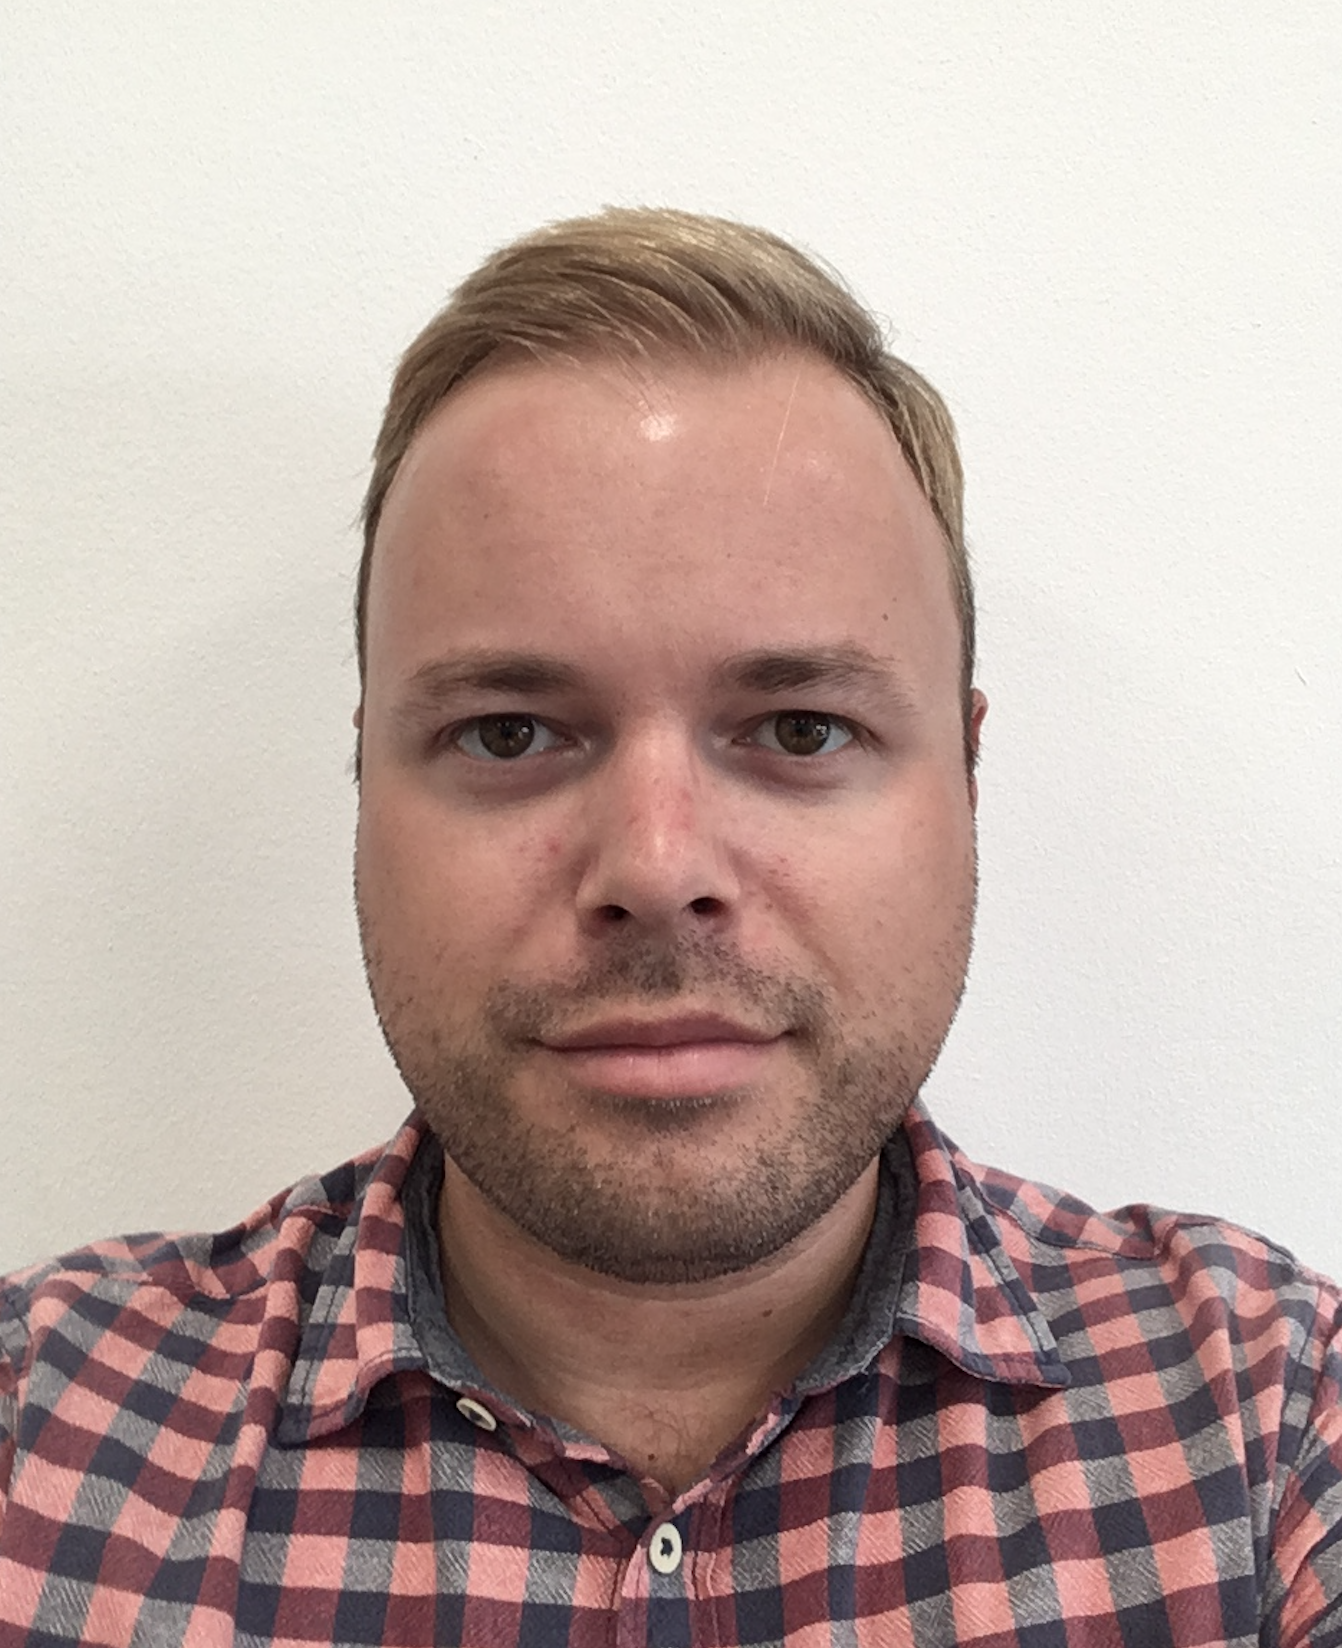
\includegraphics[width=0.20\textwidth]{me2020.png}
    \vspace*{-4cm} % avoid real text wrapping
\end{wrapfigure}

\maketitle 

%%% Personal details
\begin{minipage}[ht]{0.4\textwidth}
Shuvalovsky pr. 84 135\\
Saint-Petersburg\\
Russia\\
197345
\end{minipage}
\begin{minipage}[ht]{0.3\textwidth}
April 7th, 1986\\
+7 904 331 35 04
\end{minipage}
\vspace{10pt}

%%% About me short
\section*{Summary}
I am a bioinformatics group leader at JetBrains Research. I graduated from Saint-Petersburg State University in 2008 and received Master degree with honors in Computer Science. I'm working on computational algorithms and methods for epigenetic data analysis in the field of human aging with a specific focus on ChIP-seq and ATAC-seq methods. At the moment I am a PhD candidate under supervision of Maxim Artyomov.

%%% Research experience
\section*{Research Experience}
\begin{tabular}{L!{\VRule}R}
2017 -- today & \textbf{Visiting Research Scientist}\\
& \textit{Department of Pathology and Immunology, Washington University School of Medicine,} \\
& \textit{St. Louis, MO, USA}\\[5pt]
& Working on applied machine learning approaches and methods for epigenetic data analysis together with Maxim Artyomov Lab.\\
& \setlist{nolistsep}
\begin{itemize}[noitemsep]
  \item Developed scalable, reproducible computational pipelines for ChIP-seq processing
  \item Created pipelines for single cell ATAC-seq analysis
\end{itemize}\\

2013 -- today & \textbf{Group leader}\\
& \textit{JetBrains Research, Saint-Petersburg, Russia}\\[5pt]
& The goals of \href{http://research.jetbrains.org/groups/biolabs}{JetBrains Biolabs group} are to uncover the mechanisms underlying epigenetic regulation in humans and other animals and to identify the role of these mechanisms in cell differentiation and aging.\\
& \setlist{nolistsep}
\begin{itemize}[noitemsep]
  \item Created novel peak calling solution for ChIP-seq and ATAC-seq data analysis - semi-supervised peak caller \href{https://research.jetbrains.org/groups/biolabs/tools/span-peak-analyzer}{SPAN} and \href{https://research.jetbrains.org/groups/biolabs/tools/jbr-genome-browser}{JBR Genome Browser}
  \item Developed \href{https://research.jetbrains.org/groups/biolabs/projects?project_id=56}{Pubtrends} - exploratory tool for scientific publications providing faster trends analysis and breakthrough papers discovery
  \item Managed group activities and took part in other various group \href{https://research.jetbrains.org/groups/biolabs}{projects}
\end{itemize}\\
\end{tabular}

%%% Teaching experience
\section*{Teaching Experience}
\begin{tabular}{L!{\VRule}R}
2014 -- today  & \textbf{Scientific adviser}\\
& \textit{Bioinformatics Institute, Saint-Petersburg, Russia}\\
& \textit{Computer Science Center, Saint-Petersburg, Russia}\\
& \textit{Higher School of Economics, Saint-Petersburg, Russia}\\
& \setlist{nolistsep}
\begin{itemize}[noitemsep]
  \item Supervisor of two successful Masters dissertations
  \item Mentorship of various students projects
\end{itemize}\\
2019 - 2020 & \textbf{Lecturer}\\
& \textit{University ITMO, Saint-Petersburg, Russia}\\
& \setlist{nolistsep}
\begin{itemize}[noitemsep]
  \item Classes on computational epigenetics
\end{itemize}\\
2019 & \textbf{Lecturer}\\
& \textit{Bioinformatics Institute, Saint-Petersburg, Russia}\\
& \setlist{nolistsep}
\begin{itemize}[noitemsep]
  \item Seminar - advanced topics in computational epigenetics
\end{itemize}\\
2019 & \textbf{Lecturer}\\
& \textit{Systems Biology Workshop, Saint-Petersburg, Russia}\\
& \setlist{nolistsep}
\begin{itemize}[noitemsep]
  \item Full day workshop on epigenetics - from transcription regulation to data analysis and systems integration
\end{itemize}\\
2018, 2019 & \textbf{Invited speaker}\\
& \textit{Bioinformatics Institute Summer School, Russia}\\
\end{tabular}


%%% Professional experience
\section*{Professional Experience}
\begin{tabular}{L!{\VRule}R}
2006 -- 2013 & \textbf{Senior software developer}\\
& \textit{JetBrains, Saint-Petersburg, Russia}\\[5pt]
& Main focus was on the analysis of source code in programming languages, starting from lexical analysis to advanced type system development and source code semantic verifications.\\
& \setlist{nolistsep}
\begin{itemize}[noitemsep]
	\item Developed JetBrains products: flagship tool \href{https://jetbrains.com/idea}{IntellIJ IDEA}, \href{https://jetbrains.com/pycharm}{PyCharm}
	\item Maintained and developed \href{https://plugins.jetbrains.com/plugin/164?pr=idea}{IdeaVIM} plugin (vim emulation plugin, 7+mln downloads)
	\item Created \href{http://jetbrains.com/ruby}{RubyMine} Integrated Development Environment for Ruby programming language
\end{itemize}
\end{tabular}

%%% Education
\section*{Education}
\begin{tabular}{L!{\VRule}R}
2019 & Deep learning nanodegree at Udacity, certificate number: 9GSNRHUA  \\
& Machine learning, deep learning, models deployment \\ 
& \\
2016 & Systems Biology Workshop by Bioinformatics Institute, University ITMO and Artyomov Lab of Washington University in St.Louis, Saint-Petersburg, Russia \\
& System level data ranging from gene expression, RNA-, ChIP-, and exome-sequencing up to high-throughput metabolomics and network-based data integration.  \\ 
& \\
2015 & Microsoft Machine Learning and Intelligence School, Microsoft, Russia \\
& Machine learning, artificial intelligence, statistics. \\ 
& \\
2011 -- 2012 & Saint-Petersburg Academic University — Nanotechnology Research and Education Centre of the Russian Academy of Sciences, Russia\\
& Classes of bioinformatics, molecular biology, statistics. \\
& \\
2008 -- 2010 & Post graduate student (PhD) in Computer Science, Faculty of Mathematics and Mechanics, Saint-Petersburg State University, Russia \\
& \\
2003 -- 2008 & Masters in Computer Science, score 4.8 of 5. Saint-Petersburg State University, Russia \\
& Faculty of Mathematics and Mechanics, Chair of System Programming \\
\end{tabular}
 
\section*{Publications}
\begin{tabular}{L!{\VRule}R}

2020 & I. Shchukina, J. Bagaitkar, O. Shpynov  et al. "Epigenetic changes in aging human monocytes", Nature Aging, \textit{in review}, \\
& preprint \href{https://www.biorxiv.org/content/10.1101/2020.05.10.087023v1}{https://www.biorxiv.org/content/10.1101/2020.05.10.087023v1},\\
& website \href{https://artyomovlab.wustl.edu/aging/}{https://artyomovlab.wustl.edu/aging/}\\
2020 & D. Mogilenko et al. "Comprehensive profiling of aging immune system reveals clonal GZMK+ CD8 T cells as conserved hallmark of inflammaging", Immunity, \textit{in review},\\
&  website \href{https://artyomovlab.wustl.edu/immune-aging/}{https://artyomovlab.wustl.edu/immune-aging/}\\
2019 & O. Shpynov, A. Dievskii, P. Tsurinov, et al.  "Bioinformatics Institute 2018/19 project abstracts", Saint-Petersburg, Russia\\
2018 & Jeremy P., et al.  "Bhlhe40 is an essential repressor of IL-10 during Mycobacterium tuberculosis infection", Journal of Experimental Medicine\\
2015 & S. Lebedev, R. Chernyatchik, O. Shpynov "CMeth: a Bayesian semiparametric model
for differential methylation analysis", \\
& preprint \href{https://research.jetbrains.org/files/material/5eb189e5911b1.pdf}{https://research.jetbrains.org/files/material/5eb189e5911b1.pdf}
\end{tabular}

\section*{Languages}
\begin{tabular}{L!{\VRule}R}
Russian & Native\\
English & Fluent\\
\end{tabular}

\section*{Honors and Awards}
\begin{tabular}{L R}
& Graduated Saint-Petersburg State University cum laude\\
& Participated in ACM regional contests on programming as university team \\
&  Winner of Saint-Petersburg state school contests on math, physics, programming
\end{tabular}

\section*{Interests}
\begin{tabular}{L R}
	& Bioinformatics, machine learning, software development.\\
	& Traveling, hiking, snowboarding, diving, cycling, photography. \\
\end{tabular}
 
\end{document}